\documentclass[addpoints, 12pt, answers]{exam}

\usepackage{epstopdf}
\usepackage{makecell}

\usepackage{mathtools}
\usepackage{wrapfig}
\usepackage{tabularx}
\usepackage{multirow}
\usepackage{tikz}
\usepackage{circuitikz}
\usepackage{float}

\usepackage{setspace}

\usepackage[margin=1in]{geometry}
\usepackage{amsmath,amsthm,amssymb,amsfonts}

\usepackage[ruled,boxed,algo2e]{algorithm2e}
\usepackage{algorithm}
\usepackage{pifont}
\usepackage{graphicx}
\usepackage{listings}
\usepackage{color}

\usepackage{array}

\usepackage{booktabs}

\usepackage{amsmath,amscd}
\usepackage{amssymb,array}
\usepackage{amsfonts,latexsym}
\usepackage{graphicx,subfig,wrapfig}
\usepackage{times}
\usepackage{psfrag,epsfig}
\usepackage{verbatim}
\usepackage{tabularx}
\usepackage{makecell}
\usepackage{graphics}
\usepackage{caption}

\usepackage{enumerate}
\usepackage{listings}

\usepackage{ulem}
\usepackage[pagebackref=true,breaklinks=true,letterpaper=true,colorlinks=false,bookmarks=false]{hyperref}

\usepackage{multicol}

\usepackage{lastpage}

\usepackage{tabularray}
\usepackage{CJKutf8}

\newcommand{\N}{\mathbb{N}}
\newcommand{\Z}{\mathbb{Z}}

\DeclareMathOperator*{\rank}{rank}
\DeclareMathOperator*{\trace}{trace}
\DeclareMathOperator*{\acos}{acos}
\DeclareMathOperator*{\argmax}{argmax}

\renewcommand{\mathbf}{\boldsymbol}
\newcommand{\mb}{\mathbf}
\newcommand{\matlab}[1]{\texttt{#1}}
\newcommand{\setname}[1]{\textsl{#1}}
\newcommand{\Ce}{\mathbb{C}}
\newcommand{\norm}[2]{\left\| #1 \right\|_{#2}}

\newcommand{\exercise}[2]{\item[] \textbf{Exercise #1 #2}}

\lstset{frame=none,
    language=c,
    aboveskip=3mm,
    belowskip=3mm,
    showstringspaces=false,
    columns=flexible,
    basicstyle={\small\ttfamily},
    numbers=left,
    numberstyle=\tiny\color{gray},
    keywordstyle=\color{blue},
    commentstyle=\color{dkgreen},
    stringstyle=\color{mauve},
    breaklines=true,
    breakatwhitespace=true,
    tabsize=8
}

\definecolor{dkgreen}{rgb}{0,0.6,0}
\definecolor{gray}{rgb}{0.5,0.5,0.5}
\definecolor{mauve}{rgb}{0.58,0,0.82}




\pagestyle{headandfoot}
\runningheadrule
\firstpageheader{Computer Architecture I}{}{2025}
\runningheader{Email:}
{Homework 8, Page \thepage\ of \numpages}
{Computer Architecture I 2025}
\firstpagefooter{}{}{}
\runningfooter{}{}{}

\boxedpoints

\pointsinmargin



\setlength\answerlinelength{.95\linewidth}


\begin{document}
\begin{center}
    {\centering \Large Homework 8\\\vspace{.75cm}}

    \vspace{0.1cm}
    \makebox[\textwidth]{Chinese Name:\enspace \begin{CJK}{UTF8}{gbsn}杨人一\end{CJK}}\\[0.6cm]
    \makebox[\textwidth]{Pinyin Name:\enspace YANG RENYI}\\[0.6cm]
    \makebox[\textwidth]{Student ID:\enspace 2023533030}\\[0.6cm]
    \makebox[\textwidth]{E-Mail (omit ``@shanghaitech.edu.cn''):\enspace yangry2023}\\[0.5cm]

\end{center}


\begin{questions}

    \question[20] \textbf{Put T (True) or F (False) for each of following statement. [2 points each]}

    \begin{enumerate}[(1)]
        \item ( \quad ) On-chip cache has bigger capacity compared with the main memory because they are physically closer to the CPU.

        \item ( \quad ) In a Moore FSM,the output depends only on the current state; in a Mealy FSM, the output depends on both the current state and the inputs.

        \item ( \quad ) Assign the base address of array X to register t0. The instruction lw a0,4(t0) will always load X[1] into a0.

        \item ( \quad ) Register a0-a7 can not be changed during execution of a function.

        \item ( \quad ) Pseudo instructions could be output by the compiler.

        \item ( \quad ) The linker finalizes destination addresses for all jump instruction.

        \item ( \quad ) Spatial locality refers to the phenomenon where accessing a specific memory location makes accessing proximate storage positions more likely in the near future.

        \item ( \quad ) Assume that a processor has a two-level cache hierarchy. If L1 cache follows the write-through policy while the L2 cache follows the write-back policy, a write hit at L1 cache would always cause a write at L2 cache.

        \item ( \quad ) Instruction-level parallelism (ILP) techniques include Very Long Instruction Word (VLIW) and Single Instruction, Multiple Data (SIMD).

        \item ( \quad ) A page fault occurs if a page table entry can not be found in the TLB.

    \end{enumerate}

    \pagebreak

    \question \textbf{Number Rrepresentation [12 points]}
    \begin{parts}

        \part[6] Assume the horizontal axis represents a bit string incrementing from 00000000 to 11111111, while the vertical axis represents a decimal number. There are four different number representation. Please draw the lines of the different number representation on the figure. (Unsigned has been provided as a sample.)


        \begin{figure}[h]
            \begin{minipage}[t]{0.35\textwidth}
                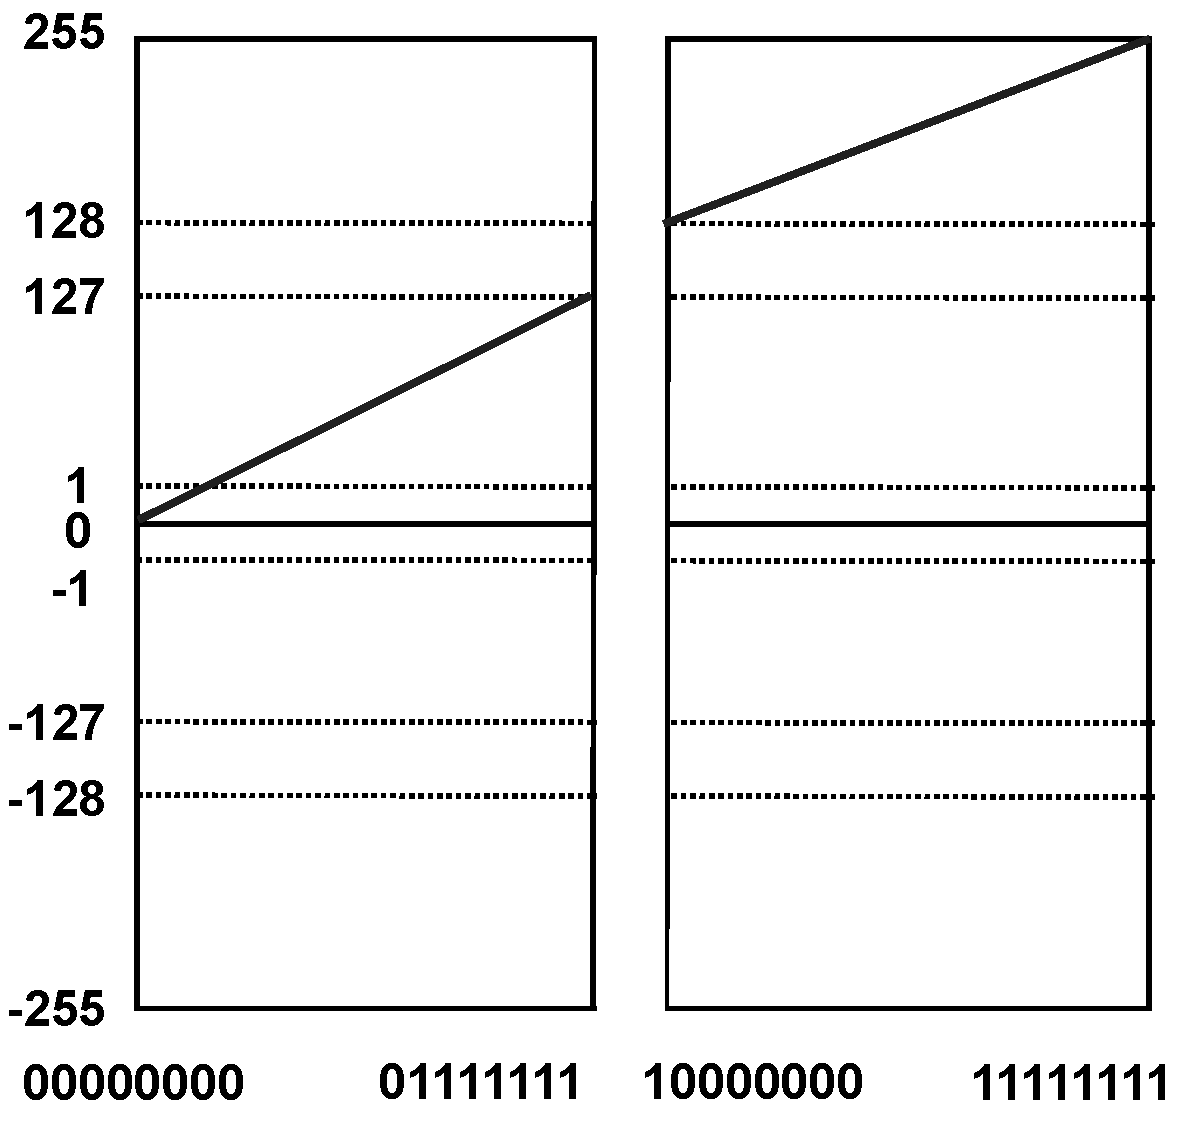
\includegraphics[width=\linewidth]{number_sample.pdf}
                \caption*{Unsigned}
            \end{minipage}
            \hfill
            \begin{minipage}[t]{0.35\textwidth}
                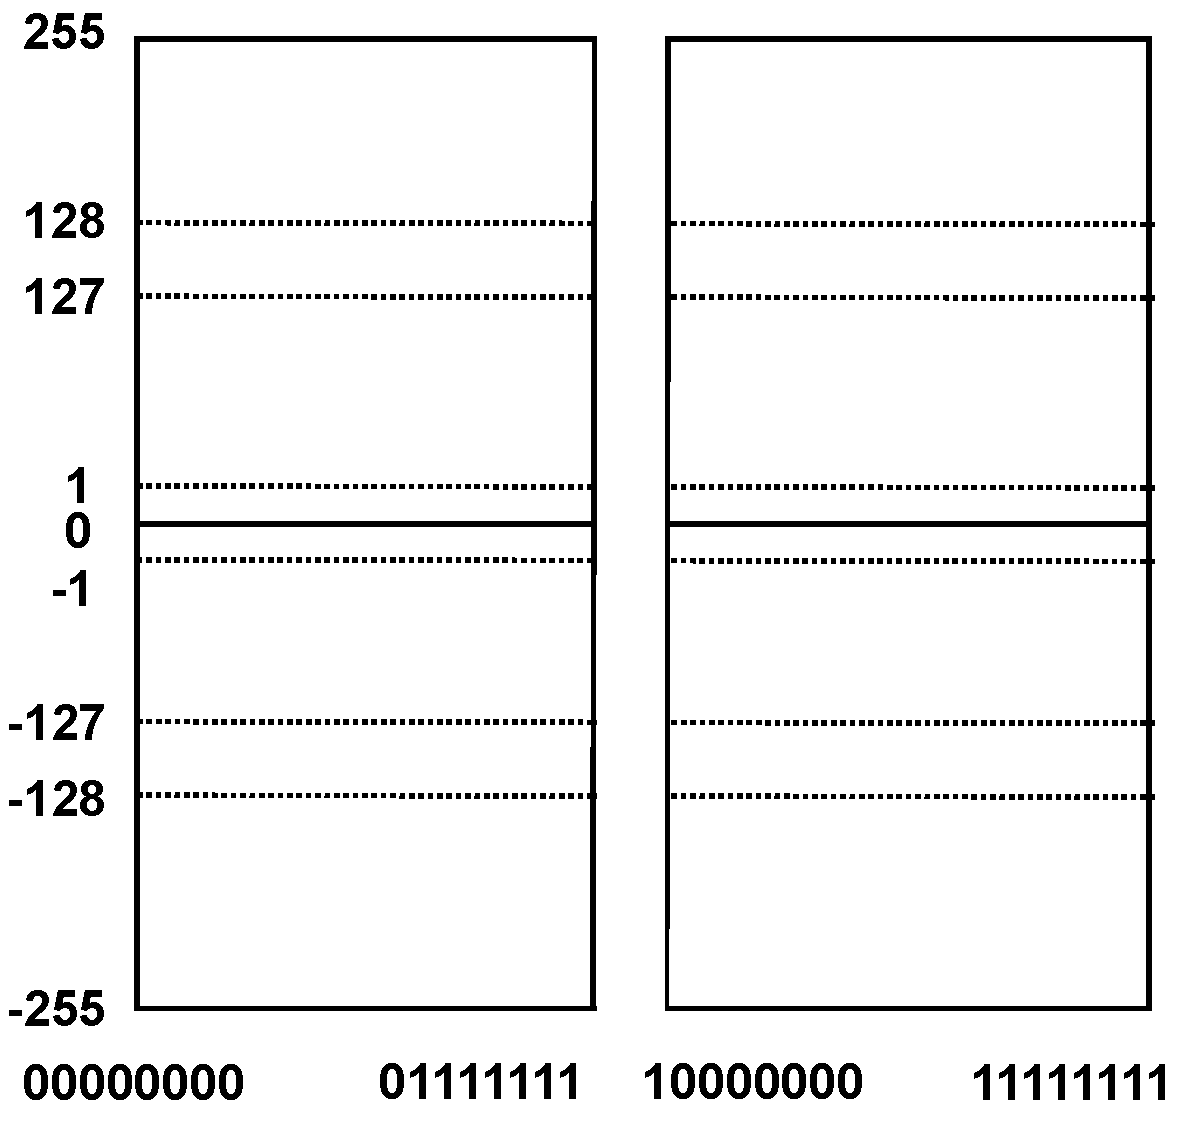
\includegraphics[width=\linewidth]{number.pdf}
                \caption*{Sign Magnitude}
            \end{minipage}
            \hfill
            \begin{minipage}[t]{0.35\textwidth}
                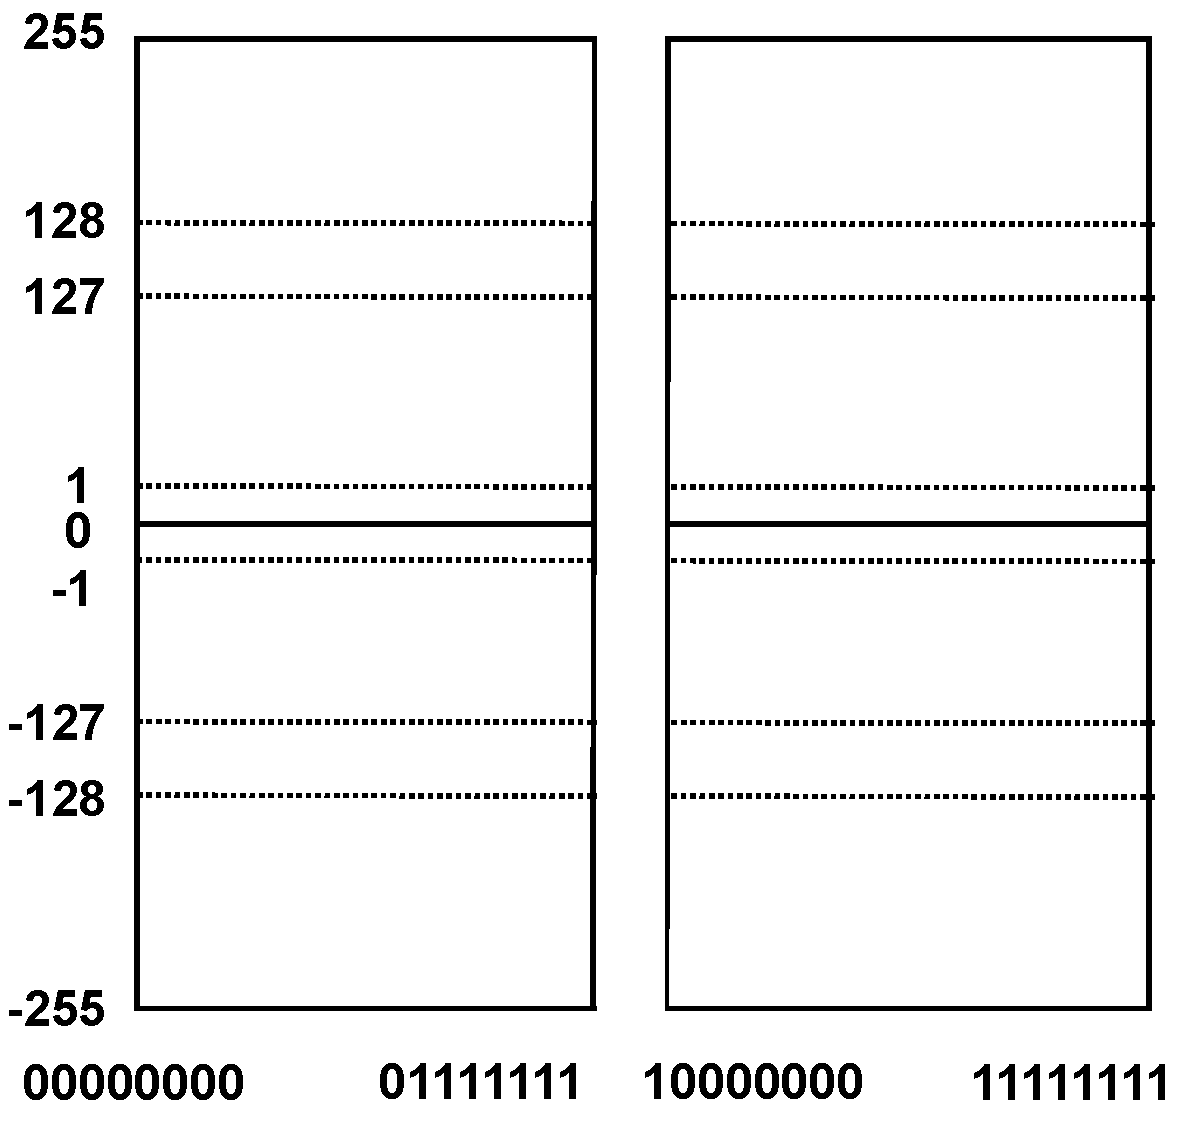
\includegraphics[width=\linewidth]{number.pdf}
                \caption*{One's complement}
            \end{minipage}
            \hfill
            \begin{minipage}[t]{0.35\textwidth}
                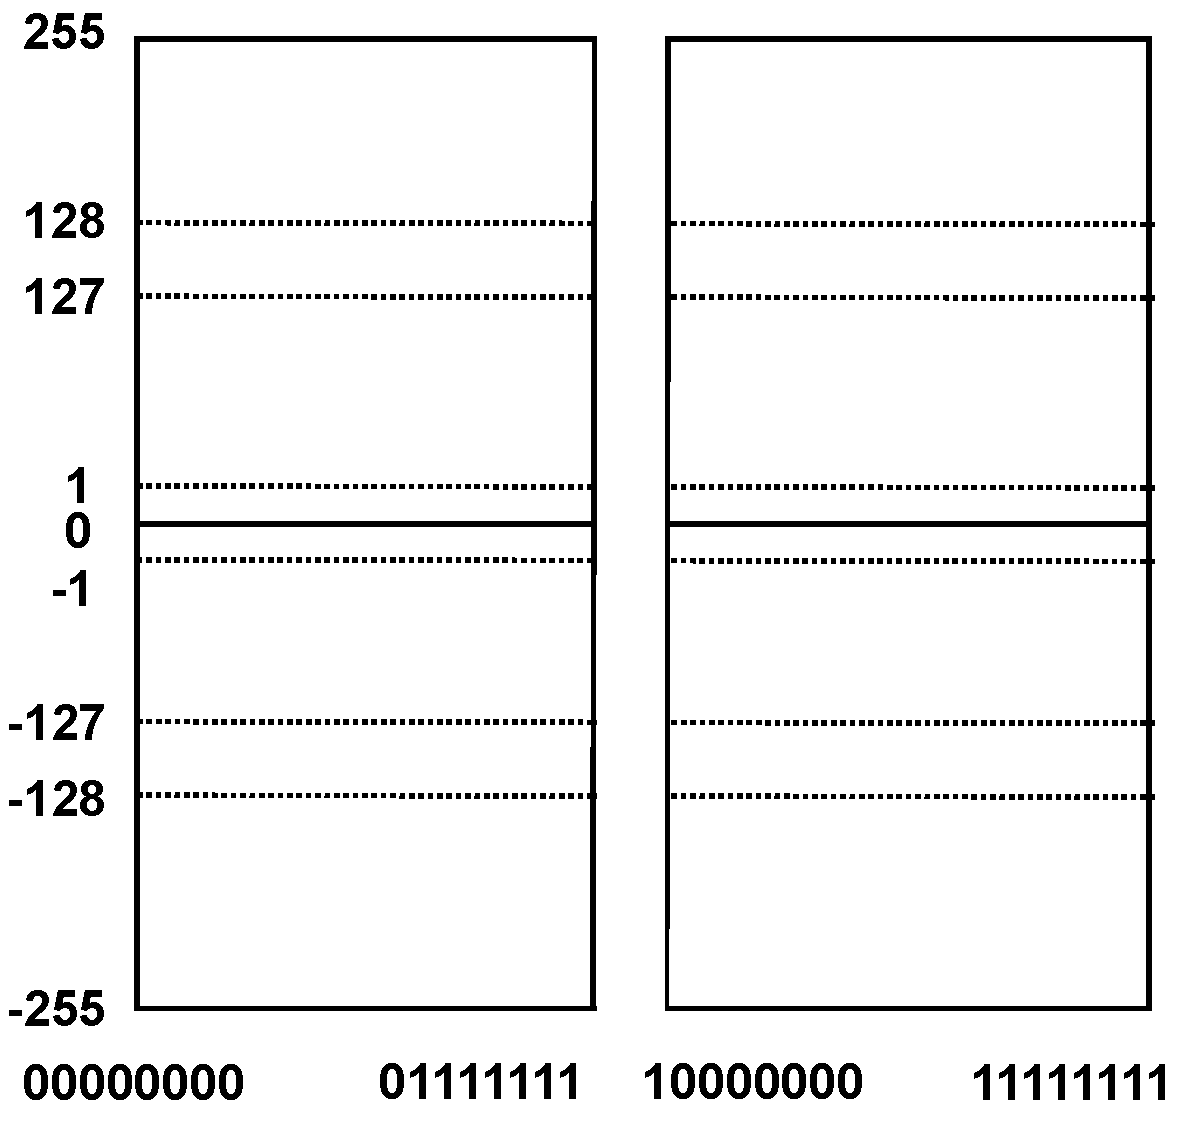
\includegraphics[width=\linewidth]{number.pdf}
                \caption*{Two's complement}
            \end{minipage}
        \end{figure}

        \part[3] What is the smallest number greater than 2 that can be represented by the IEEE 754 single-precision floating-point format?
        \\
        \\
        \\
        \part[3] What is the smallest number greater than 4 that can be represented by the IEEE 754 single-precision floating-point format?
        \\
        \\
        \\

    \end{parts}



    \pagebreak

    \question \textbf{Logic [8 points]}\\
    \begin{parts}
        \part[4] \textbf{(Multiple Choice)} Which of the following statement(s) is(are) true about boolean algebra?
        \underline{\quad\quad\quad\quad\quad\quad}
        \begin{enumerate}[A.]
            \item $XYZ+XY+X=X$.
            \item $(X+\overline{Y})X=X+X\overline{Y}$.
            \item $X+YZ=(X+Y)(X+Z)$.
            \item $(X+Y)(\overline{X}+Z)(Y+Z)=(X+Y)(\overline{X}+Z)$.
        \end{enumerate}


        \part[4] \textbf{(Multiple Choice)} Which of the following statement(s) is(are) true about boolean algebra?
        \underline{\quad\quad\quad\quad\quad\quad}
        \begin{enumerate}[A.]
            \item $X+\overline{X}Y=X+Y$.
            \item $X\overline{Y}Z+\overline{X}+Y+\overline{Z}=1$.
            \item $XY+\overline{X}Z+YZ=XY+\overline{X}Z$.
            \item $\overline{\overline{XZ+\overline{X}YZ}+\overline{Y}Z+XY\overline{Z}}=XYZ$.
        \end{enumerate}

    \end{parts}

    \question \textbf{FSM [6 points]}
    \begin{figure}[h]
        \centering
        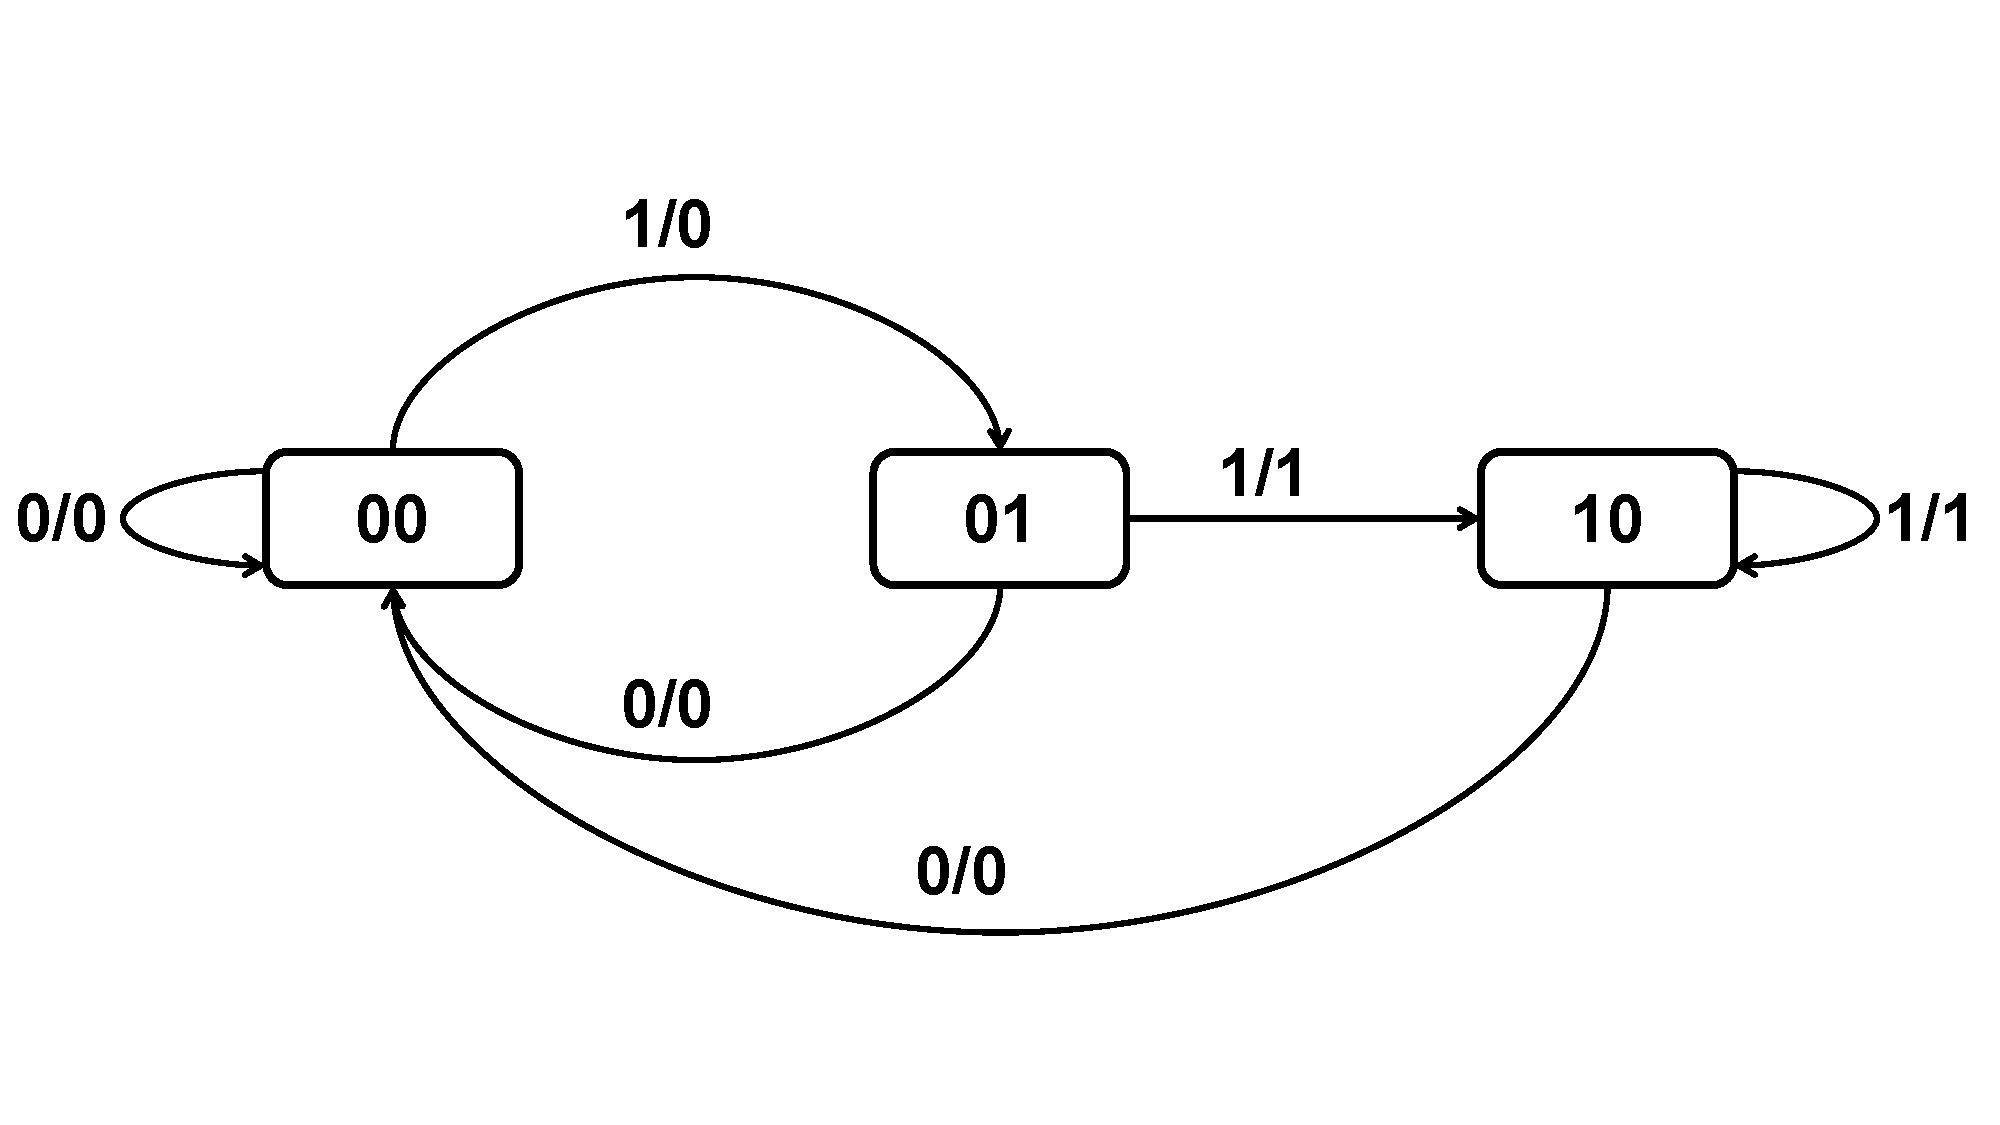
\includegraphics[width=0.5\linewidth]{fsm.pdf}
        \label{fig:fsm}
    \end{figure}

    \begin{parts}
        \part[3] Fill in the truth table for the FSM

        \begin{table}[h]
            \centering
            \begin{tabular}{|c|c|c|c|c|c|}
                \hline
                state bit 1 & state bit 0 & input & next state bit 1 & next state bit 0 & ouput \\
                \hline
                0           & 0           & 0     &                  &                  &       \\
                \hline
                0           & 0           & 1     &                  &                  &       \\
                \hline
                0           & 1           & 0     &                  &                  &       \\
                \hline
                0           & 1           & 1     &                  &                  &       \\
                \hline
                1           & 0           & 0     &                  &                  &       \\
                \hline
                1           & 0           & 1     &                  &                  &       \\
                \hline
            \end{tabular}
            \label{tab:my_label}
        \end{table}

        \part[3] Using St1(state bit 1), St0(state bit 0) and Ip(Input) as the input and Output as the output, extract a boolean expression from the truth table
        \newline

        \underline{\quad\quad\quad\quad\quad\quad\quad\quad\quad\quad\quad\quad\quad\quad\quad\quad}

    \end{parts}
    \pagebreak

    \question \textbf{C, Risc-V and Cache [23 points]}\\
    \begin{parts}
        \part[8] Suppose we have the C struct node as follows:
        {\bf\begin{lstlisting}[numbers=none]
   struct node {
    int8_t  a;
    uint8_t b;
    short   c;
    int   d;
   };
\end{lstlisting}}
        Now given N is an array, and each element of N is a pointer to struct node.
        We need to implement the following function.
            {\bf\begin{lstlisting}[numbers=none]
for(int i=0; i<length; i++) {
    N[i]->d=N[i]->a*N[i]->b+N[i]->c;
}
\end{lstlisting}}

        Complete the following RISC-V code to implement the function, assuming machine is 32-bit.
        {\bf\begin{lstlisting}[numbers=none]
  li x12, 0x00FF0000  // base address of N
  li x13, 0x3              // assume length = 3
  li x14, 0x0              // int i = 0
  j end
loop:
\end{lstlisting}}


        \underline{\quad\quad\quad\quad\quad\quad\quad\quad\quad\quad\quad\quad}\\
        \underline{\quad\quad\quad\quad\quad\quad\quad\quad\quad\quad\quad\quad}\\
        \underline{\quad\quad\quad\quad\quad\quad\quad\quad\quad\quad\quad\quad}\\
        \underline{\quad\quad\quad\quad\quad\quad\quad\quad\quad\quad\quad\quad}\\
        \underline{\quad\quad\quad\quad\quad\quad\quad\quad\quad\quad\quad\quad}\\
        \underline{\quad\quad\quad\quad\quad\quad\quad\quad\quad\quad\quad\quad}\\
        \underline{\quad\quad\quad\quad\quad\quad\quad\quad\quad\quad\quad\quad}\\
        \underline{\quad\quad\quad\quad\quad\quad\quad\quad\quad\quad\quad\quad}\\
        \underline{\quad\quad\quad\quad\quad\quad\quad\quad\quad\quad\quad\quad}\\
        \underline{\quad\quad\quad\quad\quad\quad\quad\quad\quad\quad\quad\quad}\\
        \underline{\quad\quad\quad\quad\quad\quad\quad\quad\quad\quad\quad\quad}\\
        \underline{\quad\quad\quad\quad\quad\quad\quad\quad\quad\quad\quad\quad}\\

        {\bf\begin{lstlisting}[numbers=none]
  addi x14, x14, 1
end:
  blt x14, x13, loop
  ...
\end{lstlisting}}

        \pagebreak

        \part[6] Suppose we have the following memory space before running the above program. If the machine is {\bf little-endian}, what does the memory space look like after running the program? If the machine is {\bf big-endian}, what does the memory space look like after running the program?

        Please fill in the results in the corresponding table locations.



        \begin{table}[h]
            \vspace{1em}
            \renewcommand{\arraystretch}{1.5}
            \begin{minipage}[t]{0.5\textwidth}
                \centering
                \begin{tabular}{l|l|}
                    \cline{2-2}
                    \raisebox{2ex}[0pt][0pt]{0xFFFFFFFF}  & {\bf... ...} \\ \cline{2-2}
                                                          & 0x00000C88   \\ \cline{2-2}
                                                          & 0x0000CC08   \\ \cline{2-2}
                                                          & 0x0000CC00   \\ \cline{2-2}
                    \raisebox{2ex}[0pt][0pt]{0x00FF0000}  & {\bf... ...} \\ \cline{2-2}
                                                          &              \\ \cline{2-2}
                                                          & 0xA608FA1D   \\ \cline{2-2}
                                                          &              \\ \cline{2-2}
                                                          & 0x94AE4092   \\ \cline{2-2}
                    \raisebox{2ex}[0pt][0pt]{0x0000CC00}  & {\bf... ...} \\ \cline{2-2}
                                                          &              \\ \cline{2-2}
                    \raisebox{-2ex}[0pt][0pt]{0x00000C88} & 0x1FB19515   \\ \cline{2-2}
                    \raisebox{-2ex}[0pt][0pt]{0x00000000} & {\bf... ...} \\ \cline{2-2}
                \end{tabular}
                \caption*{Little-Endian}
            \end{minipage}
            \hfill
            \begin{minipage}[t]{0.5\textwidth}
                \centering
                \begin{tabular}{l|l|}
                    \cline{2-2}
                    \raisebox{2ex}[0pt][0pt]{0xFFFFFFFF}  & {\bf... ...} \\ \cline{2-2}
                                                          & 0x00000C88   \\ \cline{2-2}
                                                          & 0x0000CC08   \\ \cline{2-2}
                                                          & 0x0000CC00   \\ \cline{2-2}
                    \raisebox{2ex}[0pt][0pt]{0x00FF0000}  & {\bf... ...} \\ \cline{2-2}
                                                          &              \\ \cline{2-2}
                                                          & 0xA608FA1D   \\ \cline{2-2}
                                                          &              \\ \cline{2-2}
                                                          & 0x94AE4092   \\ \cline{2-2}
                    \raisebox{2ex}[0pt][0pt]{0x0000CC00}  & {\bf... ...} \\ \cline{2-2}
                                                          &              \\ \cline{2-2}
                    \raisebox{-2ex}[0pt][0pt]{0x00000C88} & 0x1FB19515   \\ \cline{2-2}
                    \raisebox{-2ex}[0pt][0pt]{0x00000000} & {\bf... ...} \\ \cline{2-2}
                \end{tabular}
                \caption*{Big-Endian}
            \end{minipage}
        \end{table}



        \part[9] Now suppose we run the above code in the above memory space {\bf twice consecutively} (starting from li x12, 0x00FF0000 and ending with blt x14, x13, loop).
        All below cahce use LRU policy.

        Suppose we now have a data cache with a size of 256 Bytes and a cache block of 8 Bytes that is direct mapped. what is the hit rate of the data cache?


        \underline{\quad\quad\quad\quad\quad\quad\quad\quad\quad\quad\quad\quad}

        Suppose we now have a data cache with a size of 256 Bytes and a cache block of 8 Bytes that is 2-ways associative. what is the hit rate of the data cache?


        \underline{\quad\quad\quad\quad\quad\quad\quad\quad\quad\quad\quad\quad}


        Suppose we now have a data cache with a size of 256 Bytes and a cache block of 16 Bytes that is 4-ways associative. what is the hit rate of the data cache?

        \underline{\quad\quad\quad\quad\quad\quad\quad\quad\quad\quad\quad\quad}




    \end{parts}

    \pagebreak


    \question \textbf{Pipeline [19 points]}

    Consider a five-stage pipelined RISC-V processor shown below:
    \begin{figure}[h]
        \centering
        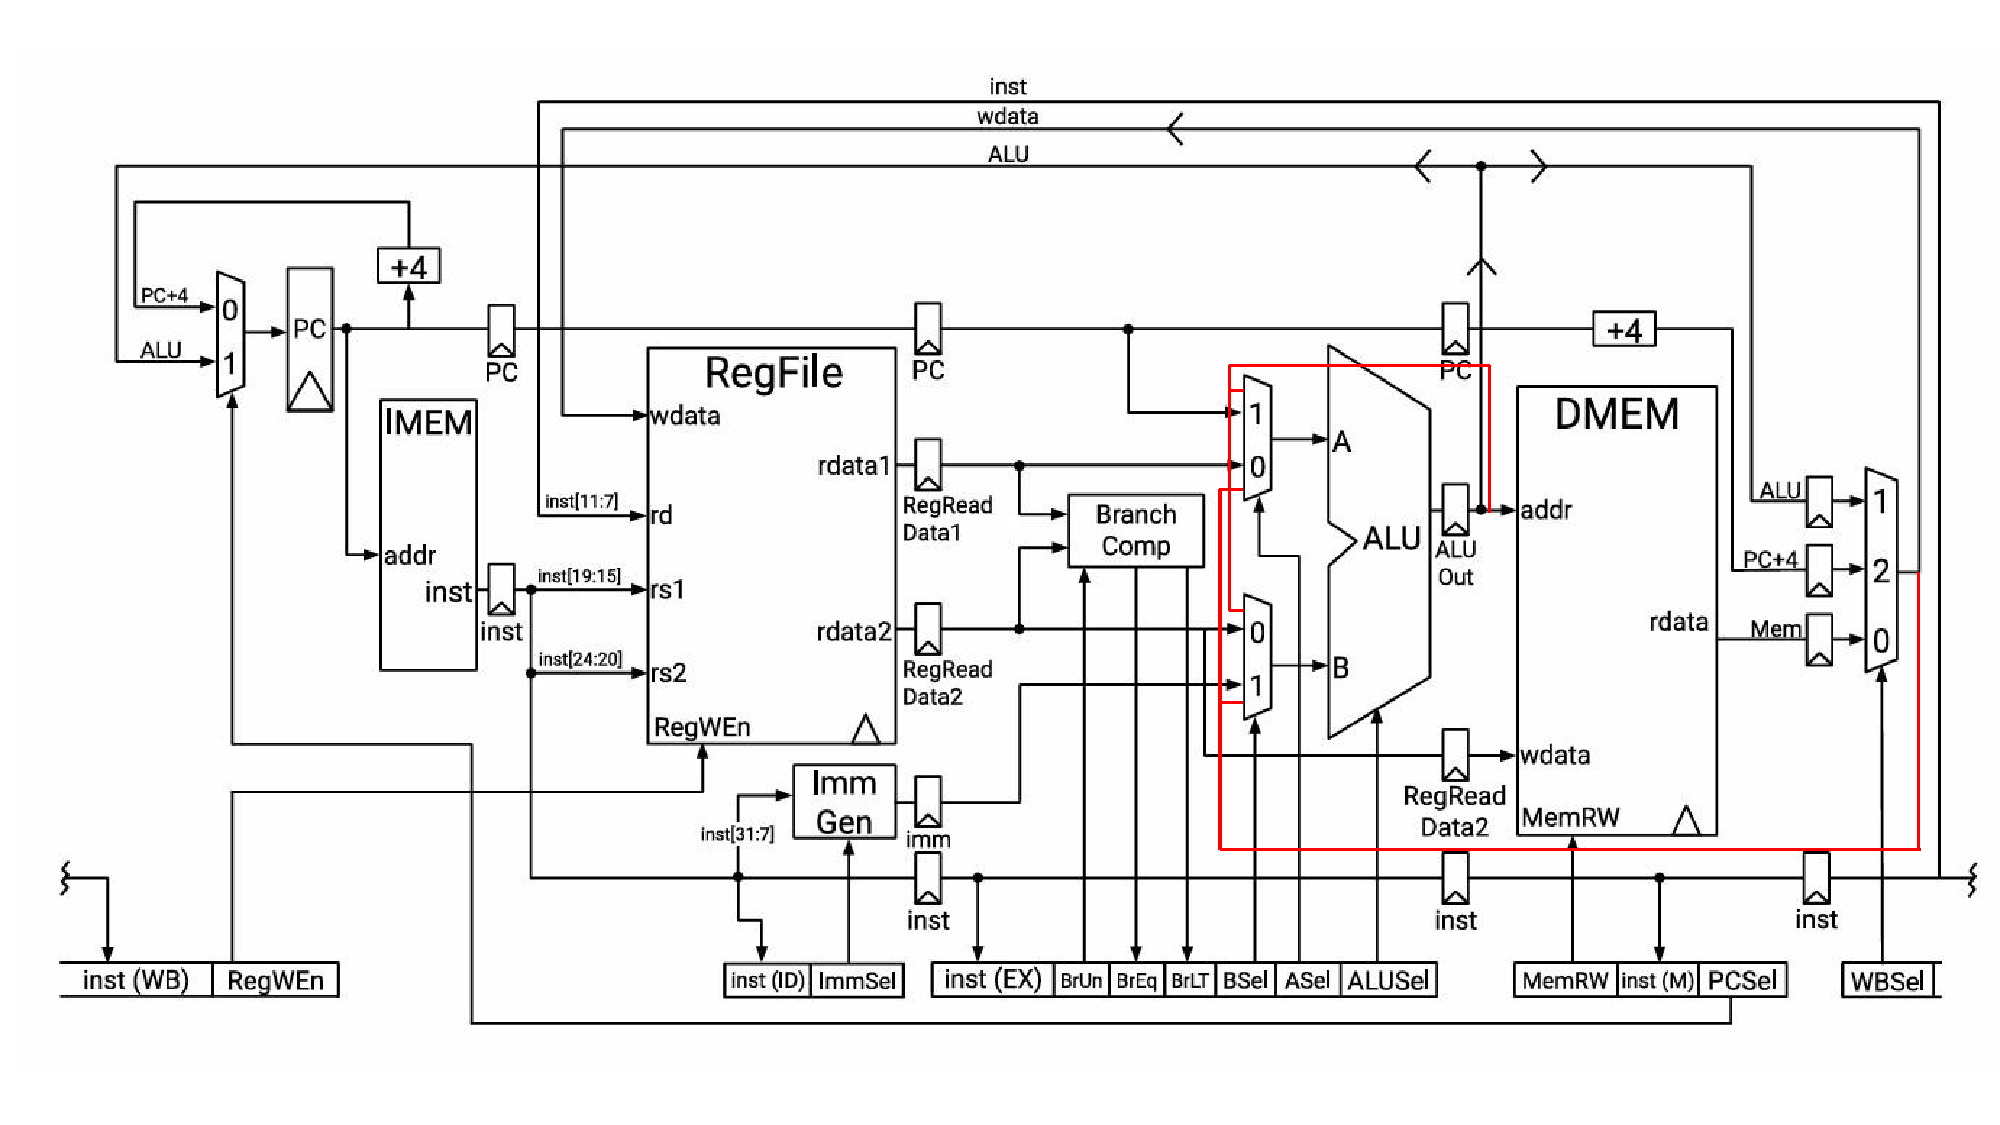
\includegraphics[width=\linewidth]{pipeline.pdf}
        \caption*{5 stage pipelined Risc-V processor}
        \label{fig:pipelined}
    \end{figure}

    Suppose that we have the following delay and setup times.

    \begin{table}[h]
        \centering
        \begin{tabular}{l l l l l l}
            {\bf Register clk-to-q} & 25ps  & {\bf Register setup}   & 25ps  & {\bf Register hold} & 5ps  \\
            {\bf RegFile read}      & 100ps & {\bf RegFile setup}    & 20ps  & {\bf Mux}           & 25ps \\
            {\bf ALU}               & 150ps & {\bf Branch comp.}     & 75ps  & {\bf Imm. Gen.}     & 15ps \\
            {\bf Memory read}       & 200ps & {\bf DMEM write setup} & 150ps                              \\
        \end{tabular}
        \label{tab:delay_time}
    \end{table}

    \begin{parts}
        \part[4] What is the highest clock frequency for this processor? Show calculation details.
        \\
        \\
        \\
        \\
        \\
        \\

        \pagebreak

        \part[4]
        If this 5 stage pipelined Risc-V processor is changed to a single-cycle datapath, what is the lowest possible $t_{clk}$? Show calculation details.
        \\
        \\
        \\
        \\
        \\

        \part[4] Forwarding datapaths are added to this five-stage pipelined RISC-V processor (the red line in Figure).
        The given code is excuted on this processor.

            {\bf    \begin{lstlisting}[label={lst:pipeline_lstlisting}]
I1:    lw   a1,  4(a0)
I2:    add  a2, a2, a0
I3:    sub  a3, a4, a1
I4:    lw   a5,  0(a1)
I5:    sub  a6, a4, a3
I6:    lw   a7,  0(a6)
I7:    add  a2, a7, a3
I8:    add  a5, a2, a4
\end{lstlisting}}

        Plese identify which instruction(s) activate the forwarding data path to reduce stall(s)? (Use $I1\rightarrow I3$, etc. to represent the instruction I1 are forward to I3.)
        \newline
        \underline{\quad\quad\quad\quad\quad\quad\quad\quad\quad\quad\quad\quad}\\
        \underline{\quad\quad\quad\quad\quad\quad\quad\quad\quad\quad\quad\quad}\\
        \underline{\quad\quad\quad\quad\quad\quad\quad\quad\quad\quad\quad\quad}\\
        \underline{\quad\quad\quad\quad\quad\quad\quad\quad\quad\quad\quad\quad}\\
        \underline{\quad\quad\quad\quad\quad\quad\quad\quad\quad\quad\quad\quad}\\
        \underline{\quad\quad\quad\quad\quad\quad\quad\quad\quad\quad\quad\quad}\\
        \part[3] With the forwarding datapaths, there is still one unavoidable stall left to correctly execute the code above. Please locate the instructions and registers that cause the stall (Use the blanks below, use I1, I2, etc. to represent the instructions).
        \newline

        The register \underline{\quad\quad\quad\quad} in instruction \underline{\quad\quad\quad\quad} and \underline{\quad\quad\quad\quad} causes the unavoidable stall.


        \part[4] Suppose we have a program with 4000 lines instructions running on this processor. What is the running time of the program ? Suppose we use the processor frequency in (a). And we assume that the CPI is the same as the CPI of the program in (c). Show calculation details.

        (Hint $\frac{time}{program}=\frac{instructions}{program}\times\frac{cycles}{instruction}\times\frac{time}{cycle}$)
        \\
        \\
        \\

    \end{parts}

    \pagebreak

    \question \textbf{AMAT and Performance [12 points]}

    \begin{parts}
        \part[4] We have a two-level cache where L1 has a hit rate of $80\%$ and a hit latency of 2 cycles, and L2 has a hit latency of $15$ cycles. Assume $100$ total accesses to this two-level cache will cause {\bf five} L2 misses on average, what is the L2 local miss rate?  Assume access to main memory takes 100 cycles, what is the Average Memory Access Time (AMAT) of this system?
        \\
        \\
        \\
        \\
        \\

        \part[4] Now we add a L3 cache to the above two-levels cache. If the hit latency of L3 cache is 30 cycles, what is the maximal local miss rate of L3 cache if we want to reduce the AMAT of the system to $8$ cycles?
        \\
        \\
        \\
        \\
        \\

        \part[4] Assume that you are given a program, of which a fraction $f$ (measured in percentage) can be optimized for parallel computing by employing N machines built as a cluster. Consider that $f=80\%$
        . If you want to accelerate the program's performance to about 3 times, what is the minimal number of N you need to employ?
        \\
        \\
        \\


    \end{parts}






\end{questions}


\end{document}
